\documentclass[a4paper,11pt,onecolumn,oneside,UTF8]{article}

\usepackage{ctex}     % 中文支持
\usepackage{amsthm,amsmath,amssymb}
\usepackage{mathrsfs}
\usepackage{bm}       % 公式中的粗体字符(用命令\boldsymbol)
\usepackage{graphicx, subfig}
\usepackage{caption}
\usepackage{float}
\usepackage{color}
\usepackage{enumerate}
\usepackage{multirow}
\usepackage{pgfplots}
\usepackage{tikz}
\usepackage{listings}
\usepackage[colorlinks,linkcolor=blue]{hyperref}

\addtolength{\topmargin}{-54pt}
\setlength{\oddsidemargin}{-0.9cm}  % 3.17cm - 1 inch
\setlength{\evensidemargin}{\oddsidemargin}
\setlength{\textwidth}{18.00cm}
\setlength{\textheight}{24.00cm}    % 24.62
\lstset{
 columns=fixed,       
 frame=none,                                          % 不显示背景边框
 backgroundcolor=\color[RGB]{245,245,244},            % 设定背景颜色
 numberstyle=\footnotesize\color{darkgray},           % 设置数字样式
 commentstyle=\it\color[RGB]{0,96,96},                % 设置代码注释的格式
 stringstyle=\rmfamily\slshape\color[RGB]{128,0,0},   % 设置字符串格式
 showstringspaces=false,                              % 不显示字符串中的空格
%  language=bash,                                       % 设置语言
%  numbers=left,                                        % 在左侧显示行号
%  numberstyle=\tiny\color{gray},                       % 设定行号格式
%  keywordstyle=\color[RGB]{40,40,255},                 % 设定关键字颜色
}

\begin{document}

\begin{center}
    \Large\textbf{Answer of Assignment 4\\第 6 章: 神经网络}
\end{center}

\begin{flushright}
    2020E8017782032\_蒲尧
\end{flushright}

\section*{第一部分:计算与证明}

\begin{enumerate}
    \item
          Consider a three-layer network for classification with $n_H$ nodes in hidden layer, and $c$ nodes in
          output layer. The patterns (also say samples ) are in $d$ dimensional space. The activation
          function (or transfer function) for the nodes in the hidden layer is the sigmoid function.
          Differently, the nodes in the output layer will employ the following softmax operation as their
          activation function:
          $$
              z_j=\frac{e^{net_j}}{\sum\limits_{m=1}^ce^{net_m}},j=1,2,...,c
          $$
          Where $net_j$ stands for the weighted sum at the \emph{j}-th node in the output layer.\\
          Please derive the learning rule under the back propagation framework if the criterion function
          for each sample is the sum of the squared errors, that is (即分析每一层权重的更新方法):
          $$
              J\left(\bm w\right)=\frac{1}{2}\sum\limits_{j=1}^c\left(t_j-z_j\right)^2
          $$
          Where $t_j$ is the known target value for the sample at the \emph{j}-th node in the output layer.\\
          注意:本题只需要推导出单个样本对权重更新的贡献即可(因为多个样本只是简单地相加)
    \item 请对反向传播算法的训练步骤进行总结;结合三层网络给出不超过三个有关权重更新的公式,并用文字
          描述所述公式的含义;指出哪些因素会对网络的性能产生影响。

\end{enumerate}

\section*{第二部分: 计算机编程}

本题使用的数据如下:\\
\begin{lstlisting}
第一类 10 个样本(三维空间):
    [ 1.58, 2.32, -5.8], [ 0.67, 1.58, -4.78], [ 1.04, 1.01, -3.63],
    [-1.49, 2.18, -3.39], [-0.41, 1.21, -4.73], [1.39, 3.16, 2.87],
    [ 1.20, 1.40, -1.89], [-0.92, 1.44, -3.22], [ 0.45, 1.33, -4.38],
    [-0.76, 0.84, -1.96]
第二类 10 个样本(三维空间):
    [ 0.21, 0.03, -2.21], [ 0.37, 0.28, -1.8], [ 0.18, 1.22, 0.16],
    [-0.24, 0.93, -1.01], [-1.18, 0.39, -0.39], [0.74, 0.96, -1.16],
    [-0.38, 1.94, -0.48], [0.02, 0.72, -0.17], [ 0.44, 1.31, -0.14],
    [ 0.46, 1.49, 0.68]
第三类 10 个样本(三维空间):
    [-1.54, 1.17, 0.64], [5.41, 3.45, -1.33], [ 1.55, 0.99, 2.69],
    [1.86, 3.19, 1.51], [1.68, 1.79, -0.87], [3.51, -0.22, -1.39],
    [1.40, -0.44, -0.92], [0.44, 0.83, 1.97], [ 0.25, 0.68, -0.99],
    [ 0.66, -0.45, 0.08]
\end{lstlisting}

\begin{enumerate}
    \item
          请编写两个通用的三层前向神经网络反向传播算法程序,一个采用{\color{blue}\textbf{批量方式更新权
              重}},另一个采用{\color{blue}\textbf{单样本方式更新权重}}。其中,隐含层结点的激励函数采用{\color{blue}\textbf{双曲正切
              函数}},输出层的激励函数采用 {\color{blue}\textbf{sigmoid 函数}}。目标函数采用{\color{blue}\textbf{平方误差准则函数}}。
    \item
          请利用上面的数据验证你写的程序,分析如下几点:
          \begin{enumerate}[(a)]
              \item 隐含层不同结点数目对训练精度的影响;
              \item 观察不同的梯度更新步长对训练的影响,并给出一些描述或解释;
              \item 在网络结构固定的情况下,绘制出目标函数随着迭代步数增加的变化曲线。

          \end{enumerate}

\end{enumerate}

\section*{第一部分回答}

\begin{enumerate}
    \item
          推到如下:令对隐藏层节点的激励函数sigmoid为f(x),对输出层节点的激励函数softmax为g(x)
          $$
              \begin{aligned}
                  f\left(s\right)      & =sigmoid\left(s\right)=\frac{1}{1+e^{-s}}                                                                                                                        \\
                  f'\left(s\right)     & =\frac{e^{-s}}{\left(1+e^{-s}\right)^2}=\frac{1}{1+e^{-s}}\left(1-\frac{1}{1+e^{-s}}\right)=y\left(1-y\right)                                                    \\
                  g\left(net_j\right)  & =z_j=softmax\left(net_j\right)=\frac{e^{net_j}}{\sum\limits_{m=1}^ce^{net_m}}                                                                                    \\
                  g'\left(net_j\right) & =\frac{\partial g\left(net_j\right)}{\partial net_m} =\frac{\frac{\partial e^{net_j}}{\partial net_m}\sum-\frac{\partial \sum}{\partial net_m}e^{net_j}}{\sum^2} \\
                                       & = \frac{e^{net_j}\sum-e^{net_j}e^{net_m}}{\sum^2}                                                                                                                \\
                                       & = \frac{e^{net_j}}{\sum}\frac{\sum-e^{net_m}}{\sum}                                                                                                              \\
                                       & =z_j\left(1-z_j\right)                                                                                                                                           \\
                  E\left(w\right)^k    & =J\left(w\right)^k=\frac{1}{2}\sum\limits_{j=1}^c\left(t_j^k-z_j^k\right)^2                                                                                      \\
                                       & =\frac{1}{2}\sum\limits_{j=1}^c\left(t_j^k-g\left(net_j^k\right)\right)^2                                                                                        \\
                                       & =\frac{1}{2}\sum\limits_{j=1}^c\left(t_j^k-g\left(\sum\limits_{h=1}^{n_H}w_{hj}y_h^k\right)\right)^2                                                             \\
                                       & =\frac{1}{2}\sum\limits_{j=1}^c\left(t_j^k-g\left(\sum\limits_{h=1}^{n_H}w_{hj}f\left(net_h^k\right)\right)\right)^2                                             \\
                                       & =\frac{1}{2}\sum\limits_{j=1}^c\left(t_j^k-g\left(\sum\limits_{h=1}^{n_H}w_{hj}f\left(\sum\limits_{i=1}^{d}w_{ih}x_i^k\right)\right)\right)^2                    \\
              \end{aligned}
          $$
          隐含层到输出层
          $$
              \begin{aligned}
                  \Delta w_{hj}         & =-\eta\frac{\partial E}{\partial w_{hj}}=-\eta\sum\limits_{k}\frac{\partial E}{\partial z_{j}^k}\frac{\partial z_{j}^k}{\partial net_{j}^k}\frac{\partial net_{j}^k}{\partial w_{hj}} \\
                                        & =\eta\sum\limits_{k}\left(t_j^k-z_j^k\right)g'\left(net_j^k\right)y_h^k                                                                                                               \\
                                        & =\eta\sum\limits_{k}\delta_j^ky_h^k                                                                                                                                                   \\
                  Where\quad \delta_j^k & =\frac{\partial E}{\partial net_{j}^k}=\left(t_j^k-z_j^k\right)g'\left(net_j^k\right)=\Delta_j^kz_j^k\left(1-z_j^k\right)=\left(t_j^k-z_j^k\right)z_j^k\left(1-z_j^k\right)
              \end{aligned}
          $$
          Single sample contribution:
          $$
              \Delta w_{hj}^k =\eta\delta_j^ky_h^k=\eta\left(t_j^k-z_j^k\right)z_j^k\left(1-z_j^k\right)y_h^k
          $$
          输入层到隐含层
          $$
              \begin{aligned}
                  \Delta w_{ih}          & =-\eta\frac{\partial E}{\partial w_{ih}}                                                                                                                                                                                                                                                      \\
                                         & =-\eta\sum\limits_{k,j}\frac{\partial E}{\partial z_{j}^k}\frac{\partial z_{j}^k}{\partial net_{j}^k}\frac{\partial net_{j}^k}{\partial y_{j}^k}\frac{\partial y_{j}^k}{\partial net_{h}^k}\frac{\partial net_{h}^k}{\partial w_{ih}}                                                         \\
                                         & =\eta\sum\limits_{k,j}\left(t_j^k-z_j^k\right)g'\left(net_j^k\right)w_{hj}f'\left(net_h^k\right)x_i^k                                                                                                                                                                                         \\
                                         & =\eta\sum\limits_{k,j}\delta_j^kw_{hj}f'\left(net_h^k\right)x_i^k                                                                                                                                                                                                                             \\
                                         & =\eta\sum\limits_{k}\left[f'\left(net_h^k\right)\sum\limits_{j}\delta_j^kw_{hj}\right]x_i^k                                                                                                                                                                                                   \\
                                         & =\eta\sum\limits_{k}\delta_h^kx_i^k                                                                                                                                                                                                                                                           \\
                  Where \quad \delta_h^k & =\frac{\partial E}{\partial net_{h}^k}=f'\left(net_h^k\right)\sum\limits_{j}\delta_j^kw_{hj}=f'\left(net_h^k\right)\Delta_h^k=\underbrace{y_h^k\left(1-y_h^k\right)}_{f'\left(net_h^k\right)}\sum\limits_{j}w_{hj}\underbrace{\left(t_j^k-z_j^k\right)z_j^k\left(1-z_j^k\right)}_{\delta_j^k}
              \end{aligned}
          $$
          Single sample contribution:
          $$
              \Delta w_{ih}^k =\eta\delta_h^kx_i^k  =\eta\underbrace{y_h^k\left(1-y_h^k\right)}_{f'\left(net_h^k\right)}\sum\limits_{j}w_{hj}\underbrace{\left(t_j^k-z_j^k\right)z_j^k\left(1-z_j^k\right)}_{\delta_j^k}x_i^k
          $$
    \item
          (1)步骤:\\
          Step1:将训练集数据输入到输入层,经过隐藏层,最后达到输出层并输出结果,这是ANN的前向传播过程;\\
          Step2:由于ANN的输出结果与实际结果有误差,则计算估计值与实际值之间的误差,并将该误差从输出层向隐藏层反向传播,直至传播到输入层;\\
          Step3:在反向传播的过程中,根据误差调整各级网络节点之间的权值$w_{ih1},w_{h1h2},...,w_{h(last)j}$;不断迭代上述过程,直至收敛或梯度下降小于某阈值。\\
          (2)权重更新公式:\\
          $$
              \begin{aligned}
                  w_{hj} & =w_{hj}+\eta\delta_j^ky_h^k \\
                  w_{ih} & =w_{ih}+\eta\delta_h^kx_i^k
              \end{aligned}
          $$
          $w_{hj}$隐含层和输出层节点权值,$\eta$学习率,$\delta_j^k$第k个样本对输出层第j个输出应该更新权重的贡献,$y_h^k$隐含层的第h个输出;\\
          $w_{ih}$输入层和隐含层节点权值,$\eta$学习率,$\delta_h^k$第k个样本对隐含层第h个输出应该更新权重的贡献,$x_i^k$输入层的第i个输出。\\
          具体算法见第一题。\\
          (3)会对网络性能产生影响的因素\\
          准则函数;激励函数;隐含层数;隐含层节点个数;初始权重;正则化技术;学习率;停止训练准则;等等。
\end{enumerate}

\section*{第二部分回答}
\begin{enumerate}
    \item
          主要代码
          \begin{lstlisting}[language=Python]
def forward(self, x_i):
    """
    Parameter:
        x_i: single sample
    Return:
        y_h: outputs of hidden-layer for single sample
        z_j: outputs of output-layer for single sample
    """
    # net_h = np.matmul(x_i.T, w_ih)
    net_h = x_i.T @ self.w_ih
    y_h = self.tahn_func(net_h)
    # net_j = np.matmul(y_h.T, w_hj)
    net_j = y_h.T @ self.w_hj
    z_j = self.sigmoid_func(net_j)
    return y_h, z_j

def backward(self, z_j, y_h, x_i, t, eta):
    """
    Parameters:
        z_j: outputs of output-layer for single sample
        y_h: outputs of hidden-layer for single sample
        x_i: inputs of input-layer for single sample
        t: target's label
        eta: learn rate
    Return:
        Delta_w_hj: hidden-layer-output-layer weight updating matrix
        Delta_w_ih: input-layer-hidden-layer weight updating matrix
        error: sample square error for ploting
    """
    # reshape the dimension of matrix (3, 1) (n_h, 1) (3, 1) (3, 1)
    z_j = np.reshape(z_j, (z_j.shape[0], 1))
    y_h = np.reshape(y_h, (y_h.shape[0], 1))
    x_i = np.reshape(x_i, (x_i.shape[0], 1))
    t = np.reshape(t, (t.shape[0], 1))
    # The following matrixs' shape: (1, 1)(3, 1)(n_h, 3)(n_h, 1)(3, n_h)
    # output error
    error = ((t - z_j).T @ (t - z_j))[0][0]
    # sigmoid'(s) = sigmoid(s) * (1-sigmoid(s)) = z_j * (1-z_j)
    delta_j = (t - z_j) * z_j * (1-z_j)
    Delta_w_hj = eta * (y_h @ delta_j.T)
    # tanh'(s) = 1-tanh(s)^2 = 1-y_h**2
    delta_h = (((t - z_j) * z_j * (1-z_j)).T @ self.w_hj.T).T * (1-y_h**2)
    Delta_w_ih = eta * (x_i @ delta_h.T)
    return Delta_w_hj, Delta_w_ih, error
    
def train(self, bk_type, eta, epoch_num):
"""
Parameters:
    bk_type: 'single' or 'batch'
    eta: learn rate
    epoch_num: maximum iretation number
Return:
    w_ih:input-layer-hidden-layer weight finally matrix
    w_hj:hidden-layer-output-layer weight finally matrix
"""
# Stochastic Backpropagation
if bk_type == 'single':
    E = []
    for _ in range(epoch_num):
        e = []
        for idx, x_i in enumerate(self.train_data):
            # forward
            y_h, z_j = self.forward(x_i)
            # backward
            Delta_w_hj, Delta_w_ih, error = self.backward(
                z_j, y_h, x_i, self.train_label[idx], eta)
            # weight update each sample
            self.w_hj += Delta_w_hj
            self.w_ih += Delta_w_ih
            e.append(error)
        E.append(np.mean(e))

# Batch Backpropagation
if bk_type == 'batch':
    E = []
    for _ in range(epoch_num):
        e = []
        Batch_Delta_w_hj = 0
        Batch_Delta_w_ih = 0
        for idx, x_i in enumerate(self.train_data):
            # forward
            y_h, z_j = self.forward(x_i)
            # backward
            Delta_w_hj, Delta_w_ih, error = self.backward(
                z_j, y_h, x_i, self.train_label[idx], eta)
            # template weight matrix update each sample
            Batch_Delta_w_hj += Delta_w_hj
            Batch_Delta_w_ih += Delta_w_ih
            e.append(error)
        # weight matrix update each iretation
        self.w_hj += Batch_Delta_w_hj
        self.w_ih += Batch_Delta_w_ih
        E.append(np.mean(e))
    \end{lstlisting}
    \item
          \begin{enumerate}[(a)]
              \item 隐含层不同结点数目对训练精度的影响,节点数$n_h$越大,收敛越快,相同迭代步数情况下,误差越小。
              \item 梯度更新步长较小时,误差变化较小,图线较光滑,越大变化越大,图线不光滑。
              \item 在网络结构固定的情况下,绘制出目标函数随着迭代步数增加的变化曲线如下图。
          \end{enumerate}
\end{enumerate}

\begin{figure}[H]
    \centering
    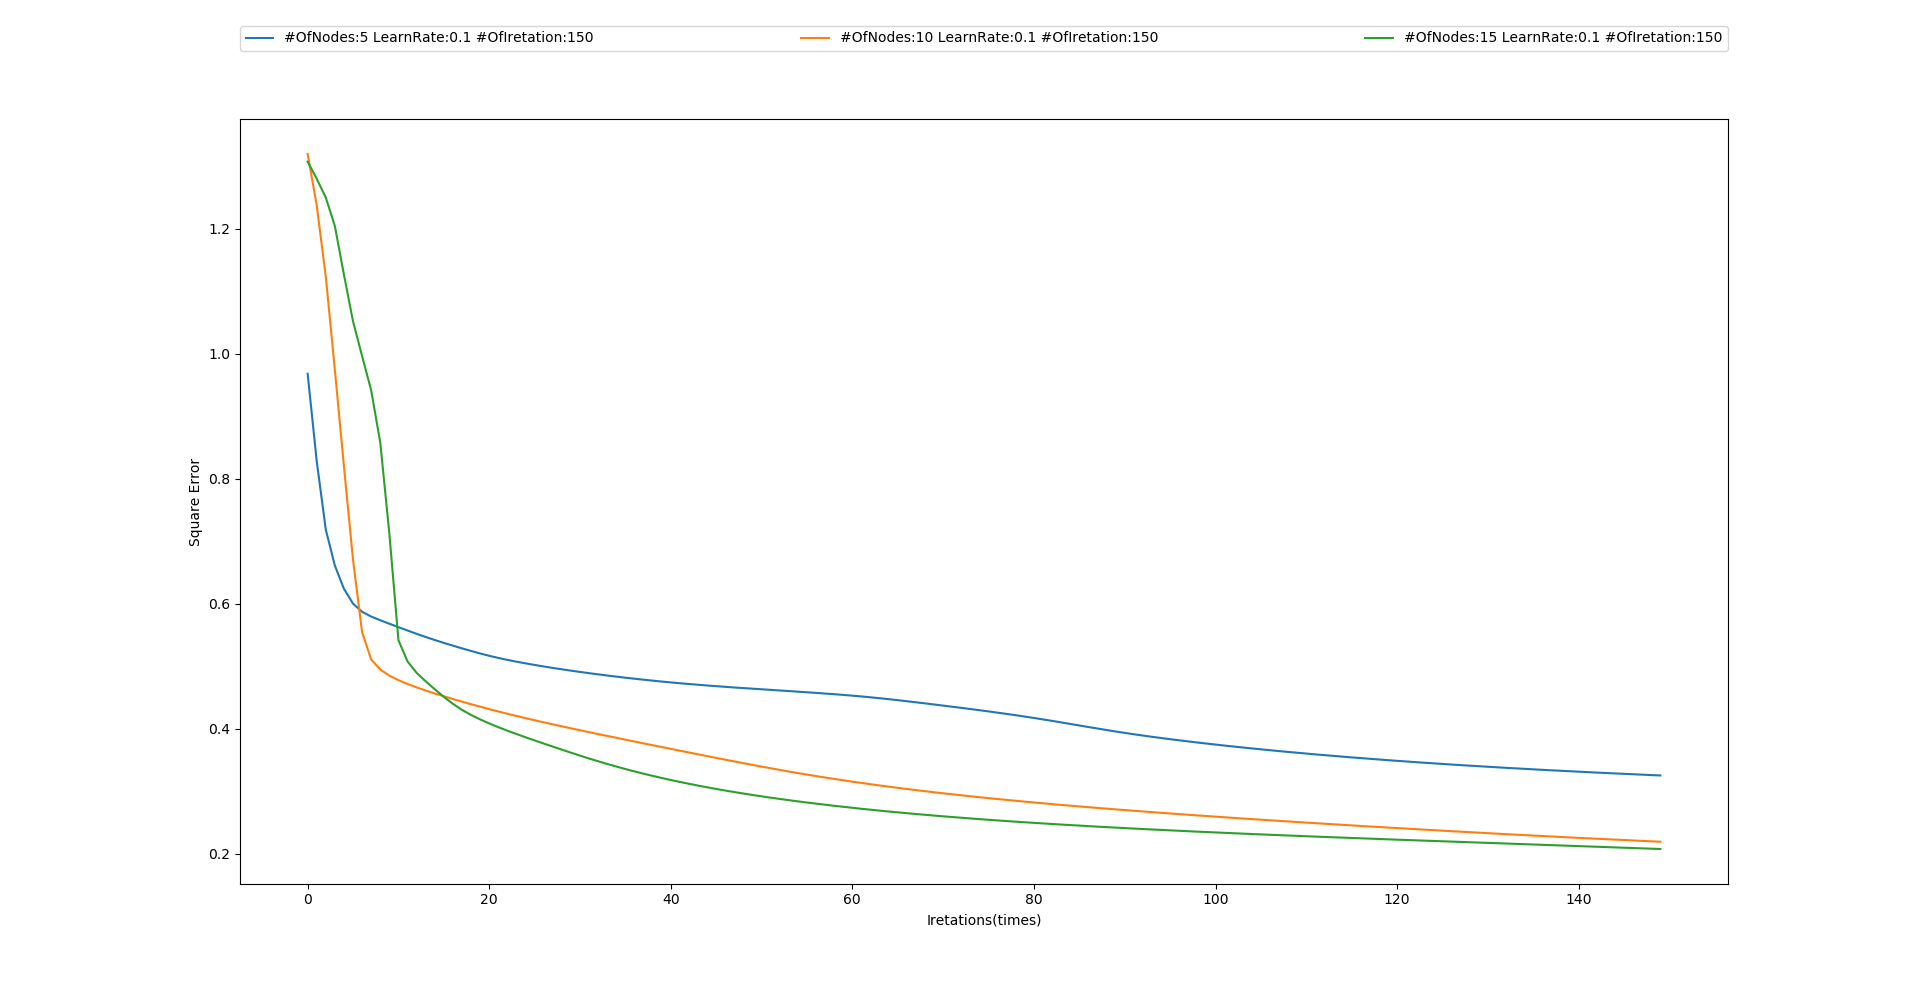
\includegraphics[width=\textwidth]{hw4_1.png}
    \caption{ 隐含层结点数目$n_h$变化对$Error$影响对比图 }
    \label{img1}
\end{figure}
\begin{figure}[H]
    \centering
    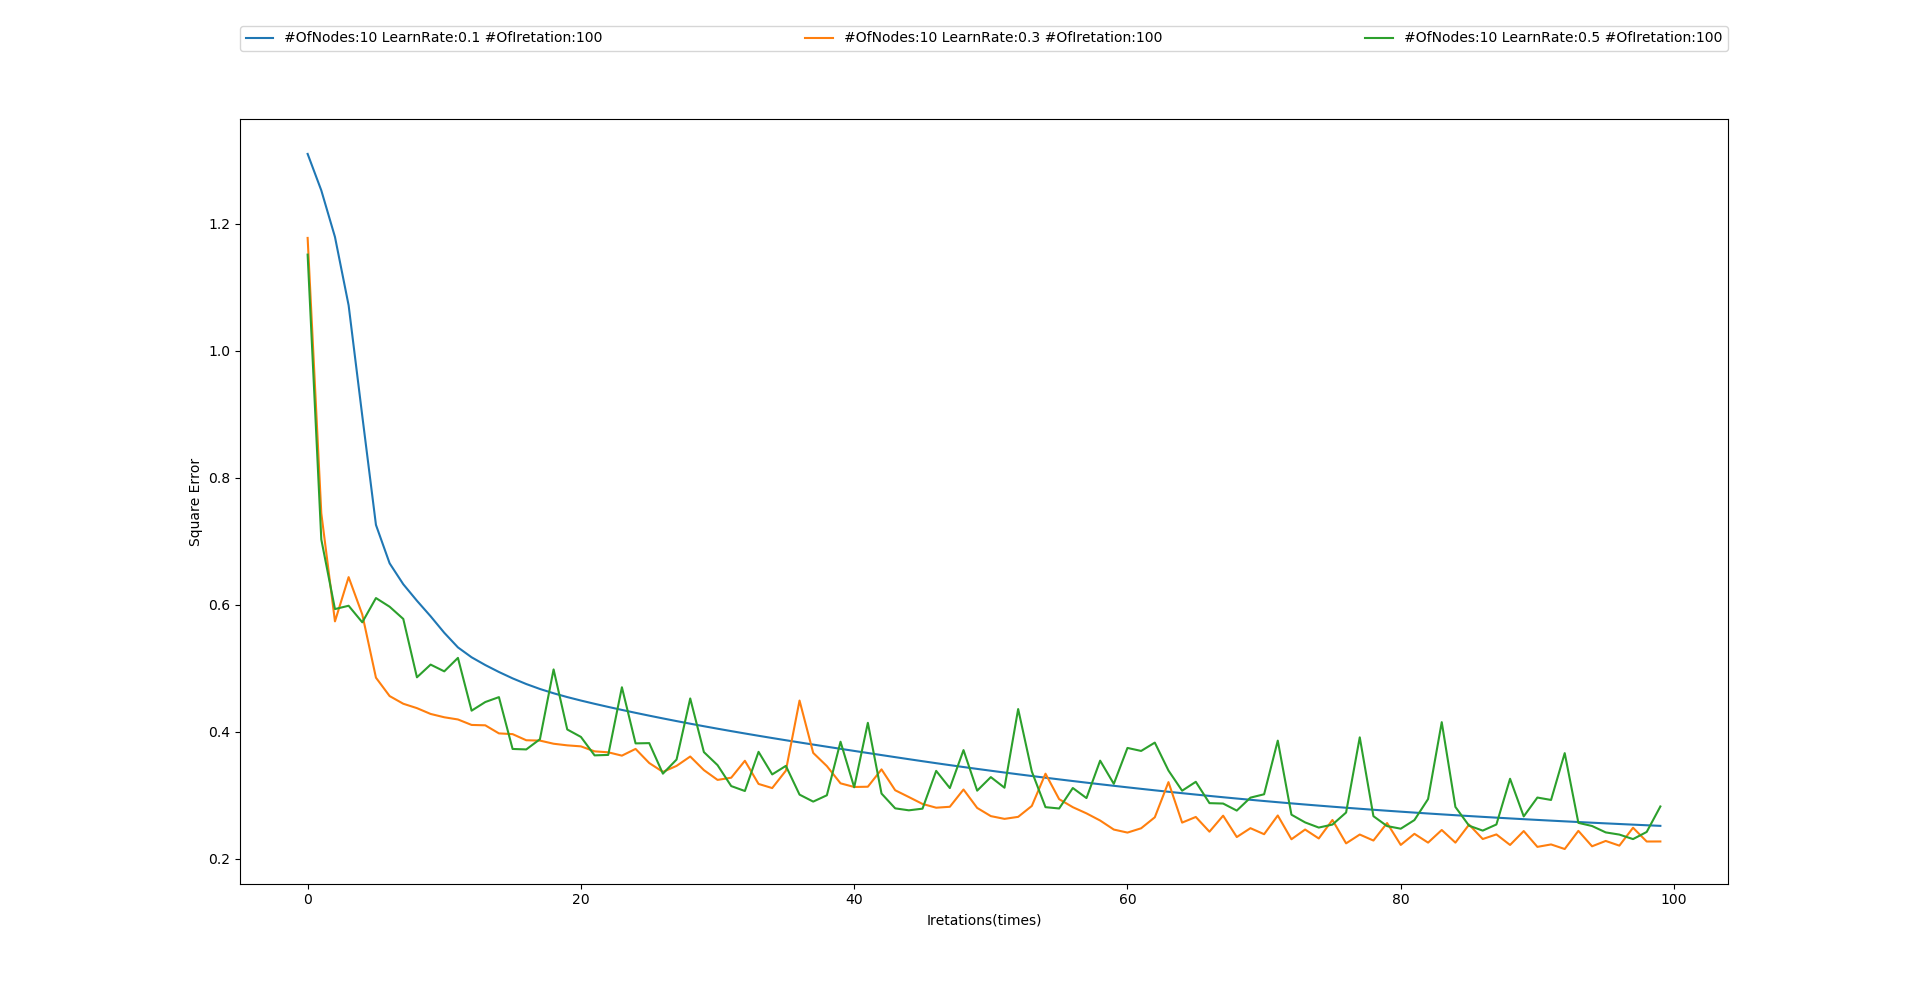
\includegraphics[width=\textwidth]{hw4_2.png}
    \caption{ 学习率$\eta$变化对$Error$影响对比图 }
    \label{img2}
\end{figure}
代码见如下文件
\href{https://github.com/Allenem/PatternRecognition/blob/main/hw4/hw4.py}{Python文件}

\end{document}